\documentclass[letterpaper,12pt]{letter}
\usepackage[letterpaper,margin=0.75in]{geometry}
\usepackage[utf8]{inputenc}
\usepackage[T1]{fontenc}
\usepackage{lmodern}
\usepackage{amsmath,amssymb}
\usepackage{enumitem}
\usepackage{tikz}
\usepackage{pgfplots}
\usepackage{setspace}
\usepackage{nopageno}
\pgfplotsset{compat=1.18}
\usetikzlibrary{arrows.meta,calc,decorations.pathmorphing,decorations.pathreplacing,decorations.markings,patterns}
\setstretch{1.18}

\begin{document}

Name: \hrulefill\ Neptun code: \hrulefill

\bigskip

\begin{center}
(KTXFI2EBNF) Physics I. Signature Retake Exam Solutions\\
May~26,~2026
\end{center}

\bigskip

\begin{enumerate}[label=\Roman*.]

\item Mechanics

\begin{enumerate}[label=\arabic*.]

\item A projectile is launched at an angle of $60^\circ$ with an initial velocity of $100\,\mathrm{m/s}$. 
Calculate:
\begin{enumerate}
    \item[(a)] The time to reach the peak of the trajectory.
    \item[(b)] The maximum height.
    \item[(c)] The horizontal range (impact distance).
    \item[(d)] The total time of flight.
\end{enumerate}
($g=9.81\,\mathrm{m/s^2}$)

\bigskip

\begin{center}
\begin{tikzpicture}[scale=0.9]
\draw[->] (0,0) -- (11,0) node[right] {$x$};
\draw[->] (0,0) -- (0,6) node[above] {$y$};

\draw[thick, blue] (0,0) parabola bend (5,5) (10,0);

\draw[->, thick, red] (0,0) -- (2,3.46);
\node[right] at (1.7,2.0) {$v_0$};

\draw[dashed] (5,0) -- (5,5);

\node at (5,-0.4) {$R$};
\node[left] at (0,5) {$h_{\max}$};

\end{tikzpicture}
\end{center}

The projectile motion can be separated into horizontal and vertical components. The horizontal velocity remains constant during the motion, while the vertical velocity changes because of gravity.

The horizontal component of the initial velocity is

$$v_{0x}=v_0\cos60^\circ=100\cdot0.5=50\,\mathrm{m/s}.$$

The vertical component of the initial velocity is

$$v_{0y}=v_0\sin60^\circ=100\cdot0.866=86.6\,\mathrm{m/s}.$$

\bigskip

\textbf{(a) Time to reach the highest point}

At the highest point of the trajectory the vertical velocity becomes zero. Therefore,

$$0=v_{0y}-gt_{\mathrm{peak}}.$$

Rearranging the equation gives

$$t_{\mathrm{peak}}=\frac{v_{0y}}{g}.$$

Substituting the numerical values,

$$t_{\mathrm{peak}}=\frac{86.6\,\mathrm{m/s}}{9.81\,\mathrm{m/s^2}}=8.83\,\mathrm{s}.$$

Therefore,

$$\boxed{t_{\mathrm{peak}}=8.83\,\mathrm{s}}.$$

\bigskip

\textbf{(b) Maximum height}

The maximum height can be calculated from the kinematic relation

$$h_{\max}=\frac{v_{0y}^2}{2g}.$$

Substituting the values,

$$h_{\max}=\frac{(86.6\,\mathrm{m/s})^2}{2\cdot9.81\,\mathrm{m/s^2}}=382\,\mathrm{m}.$$

Thus,

$$\boxed{h_{\max}=382\,\mathrm{m}}.$$

\bigskip

\textbf{(c) Horizontal range}

The total flight time is twice the time required to reach the peak:

$$t_{\mathrm{total}}=2t_{\mathrm{peak}}=2\cdot8.83\,\mathrm{s}=17.66\,\mathrm{s}.$$

The horizontal range is therefore

$$R=v_{0x}t_{\mathrm{total}}.$$

Substituting the numerical values,

$$R=50\,\mathrm{m/s}\cdot17.66\,\mathrm{s}=883\,\mathrm{m}.$$

Hence,

$$\boxed{R=883\,\mathrm{m}}.$$

\bigskip
\pagebreak
\textbf{(d) Total time of flight}

As calculated previously, the total flight time is

$$t_{\mathrm{total}}=17.66\,\mathrm{s}.$$

Therefore,

$$\boxed{t_{\mathrm{total}}=17.66\,\mathrm{s}}.$$

% -------------------------------------------------------------------------------------------------------------------

\item At what distance from the Uranus does an geosynchronous satellite orbit in the plane of the Equator if it remains constantly above the same point on the Uranus's surface? ($M_{Uranus}=8.68\cdot 10^{25}\,\mathrm{kg}$, $T_{Uranus}=-0,72 \,\mathrm{day}$, $R_{Uranus}=25300\,\mathrm{km}$, $G=6.6743\cdot 10^{-11}\,\mathrm{Nm^2/kg^2}$.)  

\bigskip

\begin{center}
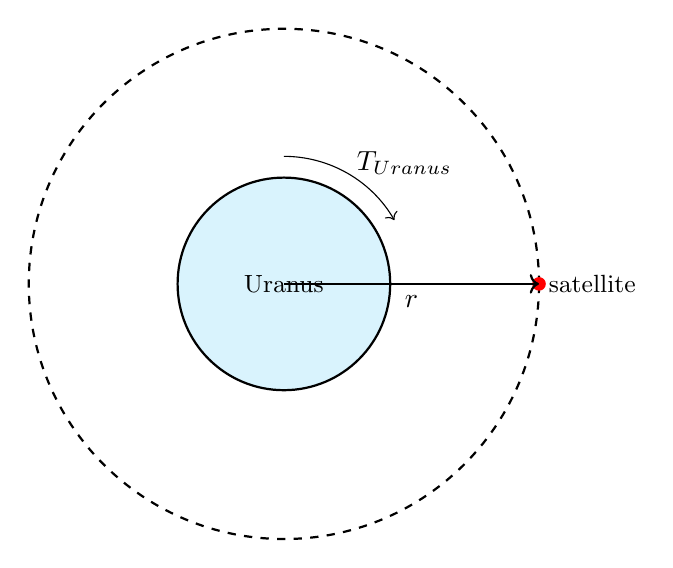
\begin{tikzpicture}[scale=0.9]
\draw[fill=cyan!15, thick] (0,0) circle (1.5);
\draw[dashed, thick] (0,0) circle (3.6);
\filldraw[red] (3.6,0) circle (2.5pt);
\draw[->, thick] (0,0) -- (3.6,0);
\node at (1.8,-0.25) {$r$};
\node at (0,0) {\small Uranus};
\node[right] at (3.6,0) {\small satellite};
\draw[->] (0,1.8) arc (90:30:1.8);
\node at (1.7,1.7) {$T_{Uranus}$};
\end{tikzpicture}
\end{center}

A geosynchronous satellite must have the same angular velocity as the rotation of Uranus. The negative sign of the given period indicates the direction of rotation, but the distance of the orbit depends on the magnitude of the period.

$$T=0.72\,\mathrm{day}=0.72\cdot24\cdot3600\,\mathrm{s}=62208\,\mathrm{s}.$$

For a circular orbit, the gravitational force provides the centripetal force:

$$\frac{GMm}{r^2}=m\frac{4\pi^2r}{T^2}.$$

The satellite mass cancels, and the orbital radius measured from the center of Uranus is

$$r=\sqrt[3]{\frac{GMT^2}{4\pi^2}}.$$

Substituting the data,

$$r=\sqrt[3]{\frac{6.6743\cdot10^{-11}\,\mathrm{Nm^2/kg^2}\cdot8.68\cdot10^{25}\,\mathrm{kg}\cdot(62208\,\mathrm{s})^2}{4\pi^2}}.$$

This gives

$$r=8.28\cdot10^7\,\mathrm{m}.$$

This is the distance from the center of Uranus. The distance from the surface is obtained by subtracting the radius of Uranus.

$$R_{Uranus}=25300\,\mathrm{km}=2.53\cdot10^7\,\mathrm{m}.$$

$$h=r-R_{Uranus}=8.28\cdot10^7\,\mathrm{m}-2.53\cdot10^7\,\mathrm{m}=5.75\cdot10^7\,\mathrm{m}.$$

Therefore the satellite orbits at the altitude

$$\boxed{h=5.75\cdot10^7\,\mathrm{m}=57500\,\mathrm{km}}.$$

The corresponding orbital radius from the center of Uranus is

$$\boxed{r=8.28\cdot10^7\,\mathrm{m}=82800\,\mathrm{km}}.$$

% -------------------------------------------------------------------------------------------------------------------

\item A $5\,\text{kg}$ object slides down from the top of a $2\text{-meter-high}$ inclined plane that makes an angle of $15^\circ$ with the horizontal. What is the velocity of the object when it reaches the bottom of the incline, starting from rest at the top, if:
\begin{enumerate}
    \item[(a)] there is no friction between the object and the incline?
    \item[(b)] the coefficient of friction is $0.2$?
\end{enumerate}
($g=9.81\,\mathrm{m/s^{2}}$)    

\bigskip

\begin{center}
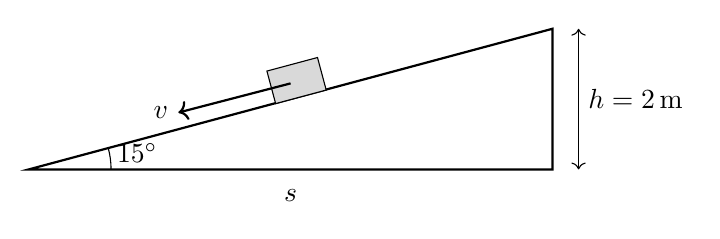
\begin{tikzpicture}[scale=0.95]
\coordinate (A) at (0,0);
\coordinate (B) at (7,0);
\coordinate (C) at (7,1.88);
\draw[thick] (A) -- (B) -- (C) -- cycle;
\draw[fill=gray!30, rotate around={15:(3.3,0.88)}] (3.3,0.88) rectangle +(0.7,0.45);
\draw[->, thick] (3.5,1.15) -- (2.0,0.76) node[left] {$v$};
\draw[<->] (7.35,0) -- (7.35,1.88);
\node[right] at (7.35,0.94) {$h=2\,\mathrm{m}$};
\draw (1.1,0) arc (0:15:1.1);
\node at (1.45,0.22) {$15^\circ$};
\node at (3.5,-0.35) {$s$};
\end{tikzpicture}
\end{center}

First, consider the case without friction. Since the object starts from rest and there is no energy loss, the initial gravitational potential energy is completely converted into kinetic energy at the bottom.

$$mgh=\frac{1}{2}mv^2.$$

The mass cancels from the equation, so the result does not depend on the mass in the frictionless case.

$$gh=\frac{1}{2}v^2.$$

Thus,

$$v=\sqrt{2gh}.$$

Substituting the values,

$$v=\sqrt{2\cdot9.81\,\mathrm{m/s^2}\cdot2\,\mathrm{m}}=6.26\,\mathrm{m/s}.$$

Therefore, without friction,

$$\boxed{v=6.26\,\mathrm{m/s}}.$$

Now consider the case with friction. The length of the inclined plane is needed because the work of friction depends on the distance travelled along the incline.

$$s=\frac{h}{\sin15^\circ}=\frac{2\,\mathrm{m}}{\sin15^\circ}=7.73\,\mathrm{m}.$$

The normal force is

$$N=mg\cos15^\circ.$$

The friction force is

$$F_f=\mu N=\mu mg\cos15^\circ.$$

The work done by friction is negative, because friction removes mechanical energy from the system.

$$W_f=-F_fs=-\mu mg\cos15^\circ s.$$

The energy equation is therefore

$$mgh-\mu mg\cos15^\circ s=\frac{1}{2}mv^2.$$

Again the mass cancels:

$$gh-\mu g\cos15^\circ s=\frac{1}{2}v^2.$$

Solving for the velocity gives

$$v=\sqrt{2gh-2\mu g\cos15^\circ s}.$$

Substituting the numerical values,

$$v=\sqrt{2\cdot9.81\,\mathrm{m/s^2}\cdot2\,\mathrm{m}-2\cdot0.2\cdot9.81\,\mathrm{m/s^2}\cdot\cos15^\circ\cdot7.73\,\mathrm{m}}.$$

This gives

$$v=3.15\,\mathrm{m/s}.$$

Therefore, with friction,

$$\boxed{v=3.15\,\mathrm{m/s}}.$$

% -------------------------------------------------------------------------------------------------------------------

\item A string is wound around a solid cylinder with radius $R = 0.6\,\text{m}$ and mass $M = 50\,\text{kg}$. Two objects with a combined mass of $25\,\text{kg}$ are hanging from the ends of the string. Upon release, the cylinder accelerates with an angular acceleration of $\beta = 5\,\text{rad/s}^2$. The string does not slip. ($g=9.81\,\mathrm{m/s^{2}}$)     
\begin{itemize}
    \item[(a)] Find the individual masses ($m_1, m_2$) of the two objects.
    \item[(b)] Calculate the total kinetic energy of the system at $t = 5\,\text{s}$.
\end{itemize}

\bigskip

\begin{center}
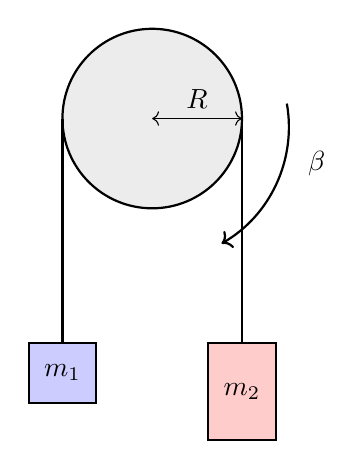
\begin{tikzpicture}[scale=0.95]
\draw[thick, fill=gray!15] (0,0) circle (1.2);
\draw[thick] (-1.2,0) -- (-1.2,-3);
\draw[thick] (1.2,0) -- (1.2,-3);
\draw[fill=blue!20, thick] (-1.65,-3.8) rectangle (-0.75,-3);
\draw[fill=red!20, thick] (0.75,-4.3) rectangle (1.65,-3);
\node at (-1.2,-3.4) {$m_1$};
\node at (1.2,-3.65) {$m_2$};
\draw[->, thick] (1.8,0.2) arc (10:-60:1.8);
\node at (2.2,-0.6) {$\beta$};
\draw[<->] (0,0) -- (1.2,0);
\node[above] at (0.6,0) {$R$};
\end{tikzpicture}
\end{center}

Since the string does not slip, the linear acceleration of the hanging masses is related to the angular acceleration of the cylinder by

$$a=R\beta.$$

Substituting the data,

$$a=0.6\,\mathrm{m}\cdot5\,\mathrm{rad/s^2}=3.0\,\mathrm{m/s^2}.$$

Let $m_2$ be the heavier mass, so that $m_2$ moves downward and $m_1$ moves upward. The equations of motion for the two hanging masses are

$$m_2g-T_2=m_2a.$$

$$T_1-m_1g=m_1a.$$

The cylinder is a solid cylinder, so its moment of inertia is

$$I=\frac{1}{2}MR^2.$$

The net torque acting on the cylinder is caused by the two string tensions:

$$(T_2-T_1)R=I\beta.$$

Substituting $I=\frac{1}{2}MR^2$ and $a=R\beta$, we get

$$T_2-T_1=\frac{1}{2}Ma.$$

From the two translational equations,

$$T_2=m_2g-m_2a=m_2(g-a).$$

$$T_1=m_1g+m_1a=m_1(g+a).$$

Therefore,

$$m_2(g-a)-m_1(g+a)=\frac{1}{2}Ma.$$

We also know that

$$m_1+m_2=25\,\mathrm{kg}.$$

Substituting the numerical values into the torque equation,

$$m_2(9.81-3.00)-m_1(9.81+3.00)=\frac{1}{2}\cdot50\cdot3.00.$$

Thus,

$$6.81m_2-12.81m_1=75.0.$$

Using $m_2=25-m_1$,

$$6.81(25-m_1)-12.81m_1=75.0.$$

Solving,

$$170.25-19.62m_1=75.0.$$

$$m_1=4.86\,\mathrm{kg}.$$

Then

$$m_2=25.0\,\mathrm{kg}-4.86\,\mathrm{kg}=20.14\,\mathrm{kg}.$$

Thus the individual masses are

$$\boxed{m_1=4.86\,\mathrm{kg}},\qquad\boxed{m_2=20.14\,\mathrm{kg}}.$$

Now calculate the kinetic energy at $t=5\,\mathrm{s}$. Since the system starts from rest and the acceleration is constant,

$$v=at=3.0\,\mathrm{m/s^2}\cdot5\,\mathrm{s}=15.0\,\mathrm{m/s}.$$

The angular velocity of the cylinder is

$$\omega=\beta t=5\,\mathrm{rad/s^2}\cdot5\,\mathrm{s}=25\,\mathrm{rad/s}.$$

The translational kinetic energy of the two masses is

$$K_{\mathrm{trans}}=\frac{1}{2}(m_1+m_2)v^2.$$

Substituting,

$$K_{\mathrm{trans}}=\frac{1}{2}\cdot25\,\mathrm{kg}\cdot(15.0\,\mathrm{m/s})^2=2812.5\,\mathrm{J}.$$

The rotational kinetic energy of the cylinder is

$$K_{\mathrm{rot}}=\frac{1}{2}I\omega^2.$$

The moment of inertia is

$$I=\frac{1}{2}MR^2=\frac{1}{2}\cdot50\,\mathrm{kg}\cdot(0.6\,\mathrm{m})^2=9.0\,\mathrm{kg\,m^2}.$$

Therefore,

$$K_{\mathrm{rot}}=\frac{1}{2}\cdot9.0\,\mathrm{kg\,m^2}\cdot(25\,\mathrm{rad/s})^2=2812.5\,\mathrm{J}.$$

The total kinetic energy is

$$K_{\mathrm{total}}=K_{\mathrm{trans}}+K_{\mathrm{rot}}=2812.5\,\mathrm{J}+2812.5\,\mathrm{J}=5625\,\mathrm{J}.$$

Thus,

$$\boxed{K_{\mathrm{total}}=5.63\cdot10^3\,\mathrm{J}}.$$

% -------------------------------------------------------------------------------------------------------------------

\pagebreak
\item Estimate the average depth of the Atlantic Ocean if a tsunami takes four hours to travel from Reykjavík to Lisbon. (Note: The propagation speed of shallow-water waves is $v=\sqrt{gh}$, where $g=9.81\,\mathrm{m/s^{2}}$. The distance is $3000$\,km.)

\bigskip

\begin{center}
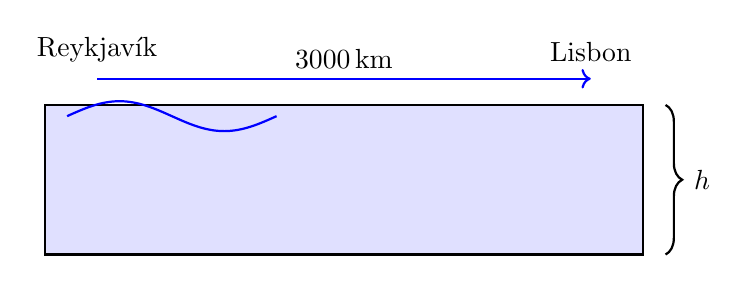
\begin{tikzpicture}[scale=0.95]
\draw[fill=blue!12, thick] (0,0) rectangle (8,-2);
\draw[thick] (0,0) -- (8,0);

\draw[thick, decorate, decoration={brace, amplitude=6pt}] (8.3,0) -- (8.3,-2);
\node[right] at (8.55,-1) {$h$};

\draw[->, thick, blue] (0.7,0.35) -- (7.3,0.35);
\node[above] at (4,0.35) {$3000\,\mathrm{km}$};

\node[above] at (0.7,0.45) {Reykjavík};
\node[above] at (7.3,0.45) {Lisbon};

\draw[thick, blue] (0.3,-0.15)
sin (1.0,0.05)
cos (1.7,-0.15)
sin (2.4,-0.35)
cos (3.1,-0.15);

\end{tikzpicture}
\end{center}

The tsunami is treated as a shallow-water wave. The propagation speed of such a wave is given by

$$v=\sqrt{gh}.$$

The travelled distance between Reykjavík and Lisbon is

$$s=3000\,\mathrm{km}=3.00\cdot10^6\,\mathrm{m}.$$

The travel time is now

$$t=4\,\mathrm{h}=4\cdot3600\,\mathrm{s}=14400\,\mathrm{s}.$$

The average propagation speed of the tsunami is therefore

$$v=\frac{s}{t}.$$

Substituting the numerical values,

$$v=\frac{3.00\cdot10^6\,\mathrm{m}}{14400\,\mathrm{s}}=208.3\,\mathrm{m/s}.$$

For shallow-water waves,

$$v=\sqrt{gh}.$$

Squaring both sides gives

$$v^2=gh.$$

Thus the average ocean depth is

$$h=\frac{v^2}{g}.$$

Substituting the values,

$$h=\frac{(208.3\,\mathrm{m/s})^2}{9.81\,\mathrm{m/s^2}}=4424\,\mathrm{m}.$$

Therefore the estimated average depth of the Atlantic Ocean is

$$\boxed{h\approx4.42\cdot10^3\,\mathrm{m}}.$$

So the estimated average depth is approximately

$$\boxed{h\approx4.4\,\mathrm{km}}.$$
\end{enumerate}

\item Thermodynamics

\begin{enumerate}[label=\arabic*.]
\setcounter{enumii}{5}

% ------------------------------------------------------------------------------------------------------------------------------------

\item We place a copper piece with a mass of 500 gramms and a temperature of $40{}^{\circ}C$ into 1250 gramms of water at $70{}^{\circ}C$. What will be the common temperature? The specific heat capacity of copper is $3.85 \cdot 10^{2}\frac{J}{kg\,K}$ and the specific heat capacity of water is $4.19 \cdot 10^{3}\frac{J}{kg\,K}$.

\bigskip

\begin{center}
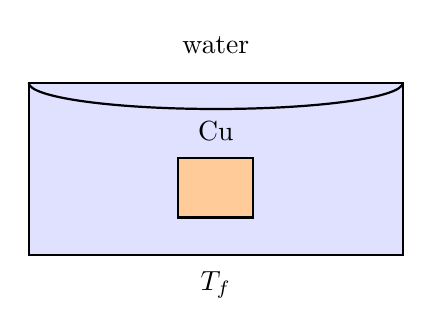
\begin{tikzpicture}[scale=0.95]
\draw[thick, fill=blue!12] (0,0) rectangle (5,2.3);
\draw[thick] (0,2.3) arc (180:360:2.5 and 0.35);
\draw[fill=orange!40, thick] (2.0,0.5) rectangle (3.0,1.3);
\node at (2.5,1.65) {Cu};
\node at (2.5,2.8) {water};
\node at (2.5,-0.4) {$T_f$};
\end{tikzpicture}
\end{center}

The water is initially hotter than the copper block, therefore thermal energy flows from the water to the copper until thermal equilibrium is reached. We assume that the system is thermally insulated, so no heat is exchanged with the environment.

The heat lost by the water is equal to the heat gained by the copper:

$$Q_{\mathrm{water}}=Q_{\mathrm{copper}}.$$

Using the calorimetric equation,

$$m_wc_w(T_w-T_f)=m_{Cu}c_{Cu}(T_f-T_{Cu}).$$

First we convert all quantities into SI units.

The mass of the copper block is

$$m_{Cu}=500\,\mathrm{g}=0.500\,\mathrm{kg}.$$

The mass of the water is

$$m_w=1250\,\mathrm{g}=1.250\,\mathrm{kg}.$$

The specific heat capacities are already given in SI units:

$$c_{Cu}=3.85\cdot10^2\,\mathrm{J/(kg\,K)}.$$

$$c_w=4.19\cdot10^3\,\mathrm{J/(kg\,K)}.$$

Substituting all numerical values into the energy balance equation,

$$1.250\,\mathrm{kg}\cdot4.19\cdot10^3\,\mathrm{J/(kg\,K)}\cdot(70-T_f)=0.500\,\mathrm{kg}\cdot3.85\cdot10^2\,\mathrm{J/(kg\,K)}\cdot(T_f-40).$$

Expanding the equation,

$$5237.5(70-T_f)=192.5(T_f-40).$$

After rearranging,

$$366625-5237.5T_f=192.5T_f-7700.$$

$$374325=5430T_f.$$

Thus,

$$T_f=68.94{}^\circ\mathrm{C}.$$

Therefore the equilibrium temperature of the system is

$$\boxed{T_f=68.9{}^\circ\mathrm{C}}.$$

% ------------------------------------------------------------------------------------------------------------------------------------

\item At a temperature of $50{}^{\circ}C$, a steel shaft with a diameter of $11.21\,cm$ needs to be fitted with an aluminum ring with an inner diameter of $11.18\,cm$ at the same temperature. The linear thermal expansion coefficient of steel is $12 \cdot 10^{-6}\frac{1}{K}$, and the linear thermal expansion coefficient of alumium is $28.7 \cdot 10^{-6}\frac{1}{K}$. What temperature should the ring be heated to?

\bigskip

\begin{center}
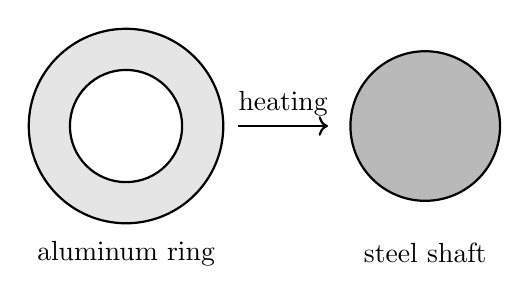
\begin{tikzpicture}[scale=0.95]
\draw[fill=gray!20, thick] (0,0) circle (1.3);
\draw[fill=white, thick] (0,0) circle (0.75);
\node at (0,-1.7) {aluminum ring};

\draw[fill=gray!55, thick] (4,0) circle (1.0);
\node at (4,-1.7) {steel shaft};

\draw[->, thick] (1.5,0) -- (2.7,0);
\node[above] at (2.1,0) {heating};
\end{tikzpicture}
\end{center}

The aluminum ring must expand sufficiently so that its inner diameter becomes equal to the diameter of the steel shaft.

The initial diameter of the aluminum ring is

$$d_0=11.18\,\mathrm{cm}=0.1118\,\mathrm{m}.$$

The required final diameter is

$$d=11.21\,\mathrm{cm}=0.1121\,\mathrm{m}.$$

The linear thermal expansion formula is

$$d=d_0(1+\alpha\Delta T).$$

The expansion coefficient of aluminum is

$$\alpha=28.7\cdot10^{-6}\,\mathrm{K^{-1}}.$$

The increase in diameter is

$$\Delta d=d-d_0=0.1121\,\mathrm{m}-0.1118\,\mathrm{m}=3.0\cdot10^{-4}\,\mathrm{m}.$$

Using the linear expansion equation,

$$\Delta d=d_0\alpha\Delta T.$$

Therefore,

$$\Delta T=\frac{\Delta d}{d_0\alpha}.$$

Substituting the numerical values,

$$\Delta T=\frac{3.0\cdot10^{-4}\,\mathrm{m}}{0.1118\,\mathrm{m}\cdot28.7\cdot10^{-6}\,\mathrm{K^{-1}}}=93.5\,\mathrm{K}.$$

The initial temperature of the ring is

$$T_0=50{}^\circ\mathrm{C}.$$

Thus the required final temperature is

$$T=T_0+\Delta T=50{}^\circ\mathrm{C}+93.5{}^\circ\mathrm{C}=143.5{}^\circ\mathrm{C}.$$

Therefore the aluminum ring should be heated to approximately

$$\boxed{T=144{}^\circ\mathrm{C}}.$$

% ------------------------------------------------------------------------------------------------------------------------------------

\pagebreak
\item The atmospheric balloon floating at an altitude of several kilometers has a volume of $1800\,m^{3}$. The temperature and pressure of the helium inside it are the same as the surrounding $-40{}^{\circ}C$ and $5 \cdot 10^{3}\,Pa$, respectively.
\begin{enumerate}
\item[(a)] How many moles of helium are in the balloon?
\item[(b)] What is the mass of the helium gas? $\left(M = 4 \frac{g}{mol}\right)$
\item[(c)] What was the volume of the balloon at the time of launch on Earth, if the gas inside the balloon was characterized by $0{}^{\circ}C$ and $10^{5}\,Pa$ pressure?
\end{enumerate}
($R=8.31\,\frac{J}{mol\cdot K}$)

\bigskip

\begin{center}
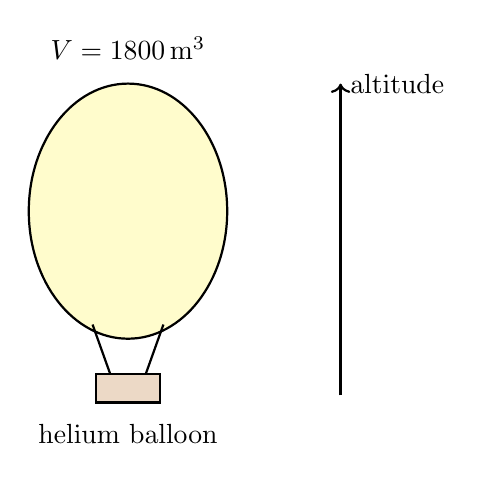
\begin{tikzpicture}[scale=0.9]
\draw[fill=yellow!20, thick] (0,0) ellipse (1.4 and 1.8);
\draw[thick] (-0.5,-1.6) -- (-0.25,-2.3);
\draw[thick] (0.5,-1.6) -- (0.25,-2.3);
\draw[fill=brown!30, thick] (-0.45,-2.7) rectangle (0.45,-2.3);

\node at (0,2.3) {$V=1800\,\mathrm{m^3}$};
\node at (0,-3.15) {helium balloon};

\draw[->, thick] (3,-2.6) -- (3,1.8);
\node[right] at (3,1.8) {altitude};
\end{tikzpicture}
\end{center}

The helium gas inside the balloon can be treated as an ideal gas. Therefore we use the ideal gas equation

$$pV=nRT.$$

The pressure is

$$p=5.0\cdot10^3\,\mathrm{Pa}.$$

The volume is

$$V=1800\,\mathrm{m^3}.$$

The temperature must be converted into kelvin:

$$T=-40{}^\circ\mathrm{C}+273.15=233.15\,\mathrm{K}.$$

\textbf{(a) Number of moles}

Rearranging the ideal gas equation,

$$n=\frac{pV}{RT}.$$

Substituting the numerical values,

$$n=\frac{5.0\cdot10^3\,\mathrm{Pa}\cdot1800\,\mathrm{m^3}}{8.31\,\mathrm{J/(mol\,K)}\cdot233.15\,\mathrm{K}}.$$

This gives

$$n=4.65\cdot10^3\,\mathrm{mol}.$$

Therefore the amount of helium inside the balloon is

$$\boxed{n=4.65\cdot10^3\,\mathrm{mol}}.$$

\textbf{(b) Mass of helium}

The molar mass of helium is

$$M=4\,\mathrm{g/mol}=4.0\cdot10^{-3}\,\mathrm{kg/mol}.$$

The mass of the helium is

$$m=nM.$$

Substituting the numerical values,

$$m=4.65\cdot10^3\,\mathrm{mol}\cdot4.0\cdot10^{-3}\,\mathrm{kg/mol}=18.6\,\mathrm{kg}.$$

Thus,

$$\boxed{m=18.6\,\mathrm{kg}}.$$

\textbf{(c) Volume at launch}

At launch conditions,

$$T_0=0{}^\circ\mathrm{C}+273.15=273.15\,\mathrm{K}.$$

$$p_0=1.0\cdot10^5\,\mathrm{Pa}.$$

The amount of helium remains constant, therefore

$$V_0=\frac{nRT_0}{p_0}.$$

Substituting the values,

$$V_0=\frac{4.65\cdot10^3\,\mathrm{mol}\cdot8.31\,\mathrm{J/(mol\,K)}\cdot273.15\,\mathrm{K}}{1.0\cdot10^5\,\mathrm{Pa}}.$$

This gives

$$V_0=105\,\mathrm{m^3}.$$

Therefore the initial volume of the balloon at launch was

$$\boxed{V_0=105\,\mathrm{m^3}}.$$

% ------------------------------------------------------------------------------------------------------------------------------------

\item The ideal cycle of an externally heated heat engine, shown in the diagram, differs from the Otto engine cycle in that it contains isothermal processes instead of adiabatic ones.

\begin{center}
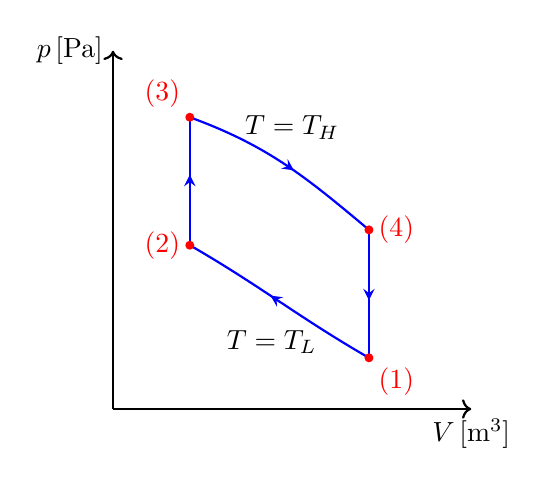
\begin{tikzpicture}[
    arrow inside/.style={
        postaction={decorate},
        decoration={
            markings,
            mark=at position 0.55 with {\arrow{stealth}}
        }
    },
scale=0.65]

    \draw[thick, ->] (0,0) -- (7,0) node[below] {$V\,\mathrm{[m^3]}$};
    \draw[thick, ->] (0,0) -- (0,7) node[left] {$p\,\mathrm{[Pa]}$};

    \coordinate (P1) at (5,1);
    \coordinate (P2) at (1.5,3.2);
    \coordinate (P3) at (1.5,5.7);
    \coordinate (P4) at (5,3.5);

    \draw[blue, thick, arrow inside] (P1) to[out=150, in=330] (P2);
    \draw[blue, thick, arrow inside] (P2) -- (P3);
    \draw[blue, thick, arrow inside] (P3) to[out=340, in=140] (P4);
    \draw[blue, thick, arrow inside] (P4) -- (P1);

    \fill[red] (P1) circle (2.5pt) node[below right] {(1)};
    \fill[red] (P2) circle (2.5pt) node[left] {(2)};
    \fill[red] (P3) circle (2.5pt) node[above left] {(3)};
    \fill[red] (P4) circle (2.5pt) node[right] {(4)};

    \node at (3.1,1.3) {$T=T_L$};
    \node at (3.5,5.5) {$T=T_H$};

\end{tikzpicture}
\end{center}

What is the efficiency of the cycle if $p_{3} = 2 p_{2}$ , the compression ratio is 8, and the cycle is performed with a two-atomic (diatomic) gas? What is the efficiency of the Carnot cycle taking place between the same temperature limits? ($R=8.31\,\mathrm{J/(mol\,K)}$)

\bigskip

The thermodynamic cycle consists of two isothermal processes and two isochoric processes.

The processes are:

\begin{itemize}
\item $1\rightarrow2$: isothermal compression,
\item $2\rightarrow3$: isochoric heating,
\item $3\rightarrow4$: isothermal expansion,
\item $4\rightarrow1$: isochoric cooling.
\end{itemize}

Because the gas is ideal, the temperature is proportional to the product $pV$:

$$T\propto pV.$$

During the isochoric process $2\rightarrow3$, the volume remains constant. Therefore,

$$\frac{T_3}{T_2}=\frac{p_3}{p_2}.$$

The problem states that

$$p_3=2p_2.$$

Thus,

$$\frac{T_3}{T_2}=2.$$

Therefore the higher temperature is twice the lower temperature:

$$T_H=T_3=T_4=2T_2=2T_L.$$

The compression ratio is defined as

$$r=\frac{V_1}{V_2}=8.$$

For a diatomic ideal gas, the molar heat capacity at constant volume is

$$C_V=\frac{5}{2}R.$$

\bigskip

\textbf{Net work of the cycle}

During an isothermal process, the work done by the gas is

$$W=nRT\ln\frac{V_f}{V_i}.$$

For the isothermal compression process $1\rightarrow2$,

$$W_{12}=nRT_L\ln\frac{V_2}{V_1}=-nRT_L\ln r.$$

For the isothermal expansion process $3\rightarrow4$,

$$W_{34}=nRT_H\ln\frac{V_4}{V_3}=nRT_H\ln r.$$

The isochoric processes do not perform mechanical work because the volume does not change.

Therefore the total work of the cycle is

$$W=W_{12}+W_{34}=nR(T_H-T_L)\ln r.$$

Since

$$T_H=2T_L,$$

we obtain

$$W=nRT_L\ln r.$$

\bigskip

\pagebreak
\textbf{Heat absorbed during the cycle}

Heat enters the system during the isochoric heating process and during the high-temperature isothermal expansion.

For the isochoric heating process,

$$Q_{23}=nC_V(T_H-T_L).$$

Using $T_H=2T_L$,

$$Q_{23}=nC_VT_L.$$

For the isothermal expansion process,

$$Q_{34}=nRT_H\ln r.$$

Thus the total absorbed heat is

$$Q_{\mathrm{in}}=nC_VT_L+nRT_H\ln r.$$

Again using $T_H=2T_L$,

$$Q_{\mathrm{in}}=nC_VT_L+2nRT_L\ln r.$$

\bigskip

\textbf{Efficiency of the engine}

The thermal efficiency is defined as

$$\eta=\frac{W}{Q_{\mathrm{in}}}.$$

Substituting the expressions derived above,

$$\eta=\frac{nRT_L\ln r}{nC_VT_L+2nRT_L\ln r}.$$

After cancellation of the common factor $nT_L$,

$$\eta=\frac{R\ln r}{C_V+2R\ln r}.$$

Using

$$C_V=\frac{5}{2}R,$$

the efficiency becomes

$$\eta=\frac{\ln r}{\frac{5}{2}+2\ln r}.$$

Since

$$r=8,$$

we have

$$\ln8=2.079.$$

Therefore,

$$\eta=\frac{2.079}{2.5+2\cdot2.079}=0.312.$$

Thus the efficiency of this heat engine cycle is

$$\boxed{\eta=0.312=31.2\%}.$$

\bigskip

\textbf{Carnot efficiency}

The Carnot efficiency between the same temperature limits is

$$\eta_C=1-\frac{T_L}{T_H}.$$

Since

$$T_H=2T_L,$$

we obtain

$$\eta_C=1-\frac{1}{2}=0.5.$$

Therefore the efficiency of the corresponding Carnot cycle is

$$\boxed{\eta_C=0.500=50.0\%}.$$

The Carnot cycle is more efficient because all heat transfer occurs reversibly at constant temperature, while in the present cycle a part of the heat transfer takes place during isochoric heating, which is thermodynamically less efficient.

% ------------------------------------------------------------------------------------------------------------------------------------

\pagebreak
\item What is the entropy change if the volume of $ m = 2\,\mathrm{g} $ of hydrogen changes from $ V_1 = 30\,\mathrm{l} \text{\ to\ } V_2 = 120\,\mathrm{l},$ and its temperature changes from $t_1 = 80^\circ\mathrm{C} \text{\ to\ } t_2 = 400^\circ\mathrm{C}$? The molar mass is $ M = 2\,\mathrm{g/mol}$, $R=8.31\,\frac{J}{mol\cdot K}$.

\bigskip

\begin{center}
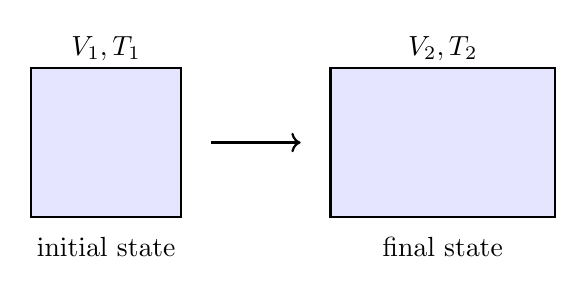
\begin{tikzpicture}[scale=0.95]
\draw[thick, fill=blue!10] (0,0) rectangle (2,2);
\draw[thick, fill=blue!10] (4,0) rectangle (7,2);

\draw[->, thick] (2.4,1) -- (3.6,1);

\node at (1,2.25) {$V_1,T_1$};
\node at (5.5,2.25) {$V_2,T_2$};

\node at (1,-0.4) {initial state};
\node at (5.5,-0.4) {final state};
\end{tikzpicture}
\end{center}

The entropy change of an ideal gas between two equilibrium states can be calculated from

$$\Delta S=nC_V\ln\frac{T_2}{T_1}+nR\ln\frac{V_2}{V_1}.$$

Hydrogen is a diatomic gas under normal conditions, therefore

$$C_V=\frac{5}{2}R.$$

The amount of substance is

$$n=\frac{m}{M}.$$

The given mass is

$$m=2\,\mathrm{g}=2.0\cdot10^{-3}\,\mathrm{kg}.$$

The molar mass is

$$M=2\,\mathrm{g/mol}=2.0\cdot10^{-3}\,\mathrm{kg/mol}.$$

Thus,

$$n=\frac{2.0\cdot10^{-3}\,\mathrm{kg}}{2.0\cdot10^{-3}\,\mathrm{kg/mol}}=1.0\,\mathrm{mol}.$$

The temperatures in kelvin are

$$T_1=80{}^\circ\mathrm{C}+273.15=353.15\,\mathrm{K}.$$

$$T_2=400{}^\circ\mathrm{C}+273.15=673.15\,\mathrm{K}.$$

The initial and final volumes converted into SI units are

$$V_1=30\,\mathrm{l}=3.0\cdot10^{-2}\,\mathrm{m^3}.$$

$$V_2=120\,\mathrm{l}=1.20\cdot10^{-1}\,\mathrm{m^3}.$$

The volume ratio is therefore

$$\frac{V_2}{V_1}=4.$$

Substituting all quantities into the entropy equation,

$$\Delta S=1.0\,\mathrm{mol}\cdot\frac{5}{2}\cdot8.31\,\mathrm{J/(mol\,K)}\cdot\ln\frac{673.15\,\mathrm{K}}{353.15\,\mathrm{K}}+1.0\,\mathrm{mol}\cdot8.31\,\mathrm{J/(mol\,K)}\cdot\ln4.$$

The temperature contribution is

$$\Delta S_T=13.4\,\mathrm{J/K}.$$

The volume contribution is

$$\Delta S_V=11.5\,\mathrm{J/K}.$$

Therefore the total entropy change is

$$\Delta S=13.4\,\mathrm{J/K}+11.5\,\mathrm{J/K}=24.9\,\mathrm{J/K}.$$

Thus the entropy increase of the hydrogen gas is

$$\boxed{\Delta S=24.9\,\mathrm{J/K}}.$$
\end{enumerate}

\item Electrostatics, Waves, and Optics

\begin{enumerate}[label=\arabic*.]
\setcounter{enumii}{10}

% ------------------------------------------------------------------------------------------------------------------------------------

\item Determine the acceleration of a proton $ m = 1.67 \cdot 10^{-27}\,\mathrm{kg} $ in an electric field of strength $ E = 300\,\mathrm{N/C}. $ How many times greater is this acceleration than the acceleration due to gravity? ($e=1.6\cdot 10^{-19}\,\mathrm{C}$, $g=9.81\,\mathrm{m/s^{2}}$)

\bigskip

\begin{center}
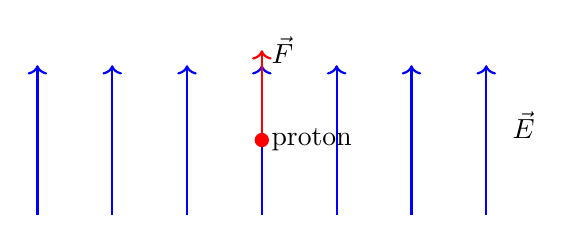
\begin{tikzpicture}[scale=0.95]

\foreach \x in {0,1,...,6}
{
\draw[->, thick, blue] (\x,0) -- (\x,2);
}

\filldraw[red] (3,1) circle (2.5pt);

\node[right] at (3,1) {proton};

\node at (6.5,1.2) {$\vec E$};

\draw[->, thick, red] (3,1) -- (3,2.2);
\node[right] at (3,2.2) {$\vec F$};

\end{tikzpicture}
\end{center}

A proton placed in an electric field experiences an electric force. The magnitude of the electric force acting on a charged particle is

$$F=qE.$$

For a proton, the electric charge is

$$q=e=1.6\cdot10^{-19}\,\mathrm{C}.$$

The electric field strength is

$$E=300\,\mathrm{N/C}.$$

Therefore the electric force acting on the proton is

$$F=(1.6\cdot10^{-19}\,\mathrm{C})(300\,\mathrm{N/C})=4.8\cdot10^{-17}\,\mathrm{N}.$$

According to Newton's second law,

$$F=ma.$$

Thus the acceleration is

$$a=\frac{F}{m}.$$

The proton mass is

$$m=1.67\cdot10^{-27}\,\mathrm{kg}.$$

Substituting the numerical values,

$$a=\frac{4.8\cdot10^{-17}\,\mathrm{N}}{1.67\cdot10^{-27}\,\mathrm{kg}}=2.87\cdot10^{10}\,\mathrm{m/s^2}.$$

Therefore the acceleration of the proton is

$$\boxed{a=2.87\cdot10^{10}\,\mathrm{m/s^2}}.$$

Now compare this acceleration to the acceleration due to gravity.

The ratio is

$$\frac{a}{g}=\frac{2.87\cdot10^{10}\,\mathrm{m/s^2}}{9.81\,\mathrm{m/s^2}}=2.93\cdot10^9.$$

Thus the electric acceleration is approximately $\boxed{2.93\cdot10^9}$ times greater than the gravitational acceleration.

% ------------------------------------------------------------------------------------------------------------------------------------

\pagebreak
\item An electron is launched with an initial velocity of $ v_0 = 3\cdot 10^6\,\mathrm{m/s} $ between two parallel charged plates, as shown in the figure. If the electric field strength between the plates is $ E = 3\,\mathrm{kN/C}, $ where does the electron hit the upper plate? Assume that the arrangement is in vacuum.

\begin{center}
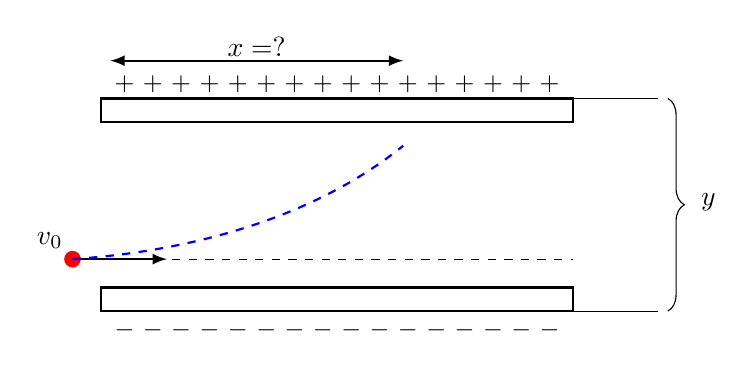
\begin{tikzpicture}[scale=1.2, >=latex]

\draw[thick] (0,0) rectangle (5,0.25);
\draw[thick] (0,-2.0) rectangle (5,-1.75);

\foreach \x in {0.25,0.55,...,5.0}
{
    \node at (\x,0.4) {\small $+$};
}

\foreach \x in {0.25,0.55,...,5.0}
{
    \node at (\x,-2.2) {\small $-$};
}

\fill[red] (-0.3,-1.45) circle (2.5pt);

\draw[->, thick] (-0.25,-1.45) -- (0.7,-1.45);
\node[left] at (-0.3,-1.25) {$v_0$};

\draw[dashed] (-0.3,-1.45) -- (5.0,-1.45);

\draw[dashed, thick, blue]
    (-0.3,-1.45) .. controls (1.2,-1.35) and (2.4,-0.9) .. (3.2,-0.25);

\draw[<->, thick] (0.1,0.65) -- (3.2,0.65);
\node at (1.65,0.8) {$x=?$};

\draw[thin] (5.6,0.25) -- (5.9,0.25);
\draw[thin] (5.6,-2.0) -- (5.9,-2.0);

\draw[decorate, decoration={brace, amplitude=6pt,mirror}]
    (6.0,-2.0) -- (6.0,0.25);

\node[right] at (6.25,-0.85) {$y$};

\draw[thin] (5.0,0.25) -- (5.6,0.25);
\draw[thin] (5.0,-2.0) -- (5.6,-2.0);

\end{tikzpicture}
\end{center}

($m_{e}=9.1\cdot 10^{-31}\,\mathrm{kg}$, $e=1.6\cdot 10^{-19}\,\mathrm{C}$)

\bigskip

The electron moves horizontally with constant velocity while simultaneously accelerating vertically because of the electric field. The motion is therefore analogous to projectile motion.

The electric field strength is

$$E=3\,\mathrm{kN/C}=3.0\cdot10^3\,\mathrm{N/C}.$$

The electric force acting on the electron is

$$F=eE.$$

Substituting the values,

$$F=(1.6\cdot10^{-19}\,\mathrm{C})(3.0\cdot10^3\,\mathrm{N/C})=4.8\cdot10^{-16}\,\mathrm{N}.$$

The acceleration of the electron is

$$a=\frac{F}{m_e}.$$

Using the electron mass,

$$m_e=9.1\cdot10^{-31}\,\mathrm{kg},$$

we obtain

$$a=\frac{4.8\cdot10^{-16}\,\mathrm{N}}{9.1\cdot10^{-31}\,\mathrm{kg}}=5.27\cdot10^{14}\,\mathrm{m/s^2}.$$

The electron starts halfway between the plates. The plate separation from the figure is

$$y=2.0\,\mathrm{cm}=2.0\cdot10^{-2}\,\mathrm{m}.$$

Therefore the vertical distance travelled before hitting the upper plate is

$$s_y=\frac{y}{2}=1.0\cdot10^{-2}\,\mathrm{m}.$$

The initial vertical velocity is zero, so the vertical motion equation is

$$s_y=\frac{1}{2}at^2.$$

Solving for the time,

$$t=\sqrt{\frac{2s_y}{a}}.$$

Substituting the numerical values,

$$t=\sqrt{\frac{2\cdot1.0\cdot10^{-2}\,\mathrm{m}}{5.27\cdot10^{14}\,\mathrm{m/s^2}}}=6.16\cdot10^{-9}\,\mathrm{s}.$$

The horizontal velocity remains constant:

$$v_0=3.0\cdot10^6\,\mathrm{m/s}.$$

Thus the horizontal distance travelled before collision is

$$x=v_0t.$$

Substituting,

$$x=(3.0\cdot10^6\,\mathrm{m/s})(6.16\cdot10^{-9}\,\mathrm{s})=1.85\cdot10^{-2}\,\mathrm{m}.$$

Therefore the electron hits the upper plate at the distance

$$\boxed{x=1.85\cdot10^{-2}\,\mathrm{m}=1.85\,\mathrm{cm}}$$

from the entrance point.

% ------------------------------------------------------------------------------------------------------------------------------------

\pagebreak
\item An electron enters the region between the plate pair shown in the figure halfway between the plates. The length of the plates is $ l = 20\,\mathrm{cm}, $ their separation is $ d = 2\,\mathrm{cm}, $ and the voltage between them is $ U = 500\,\mathrm{V}. $ What must the initial velocity of the electron be if we want it to just barely leave the region between the plates? ($m_{e}=9.1\cdot 10^{-31}\,\mathrm{kg}$, $e=1.6\cdot 10^{-19}\,\mathrm{C}$)

\begin{center}
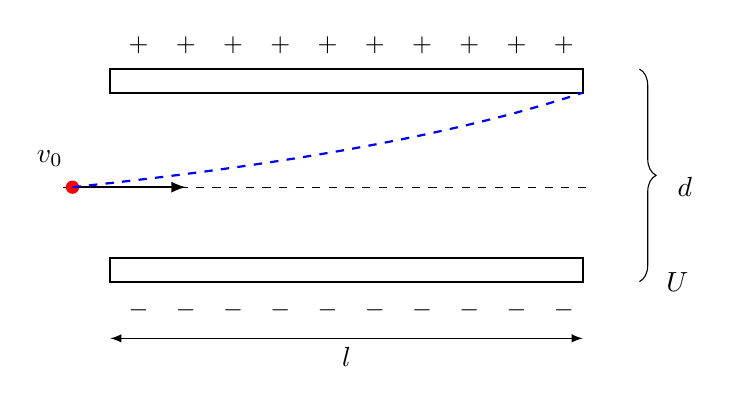
\begin{tikzpicture}[scale=1.2, >=latex]

\def\L{5}
\def\d{2}

\draw[thick] (0,0) rectangle (\L,0.25);
\draw[thick] (0,-\d) rectangle (\L,-\d+0.25);

\foreach \x in {0.3,0.8,...,4.8}
{
    \node at (\x,+0.5) {\small $+$};
}

\foreach \x in {0.3,0.8,...,4.8}
{
    \node at (\x,-2.3) {\small $-$};
}

\draw[dashed] (-0.5,-\d/2) -- (\L+0.1,-\d/2);

\fill[red] (-0.4,-\d/2) circle (2pt);

\draw[->, thick] (-0.4,-\d/2) -- (0.8,-\d/2);
\node[left] at (-0.4,-\d/2+0.3) {$v_0$};

\draw[thick, dashed, blue]
    (-0.4,-\d/2) .. controls (1.5,-\d/2+0.2) and (3.5,-0.5) .. (\L,0.0);

\draw[<->] (0,-\d-0.6) -- (\L,-\d-0.6);
\node at (\L/2,-\d-0.8) {$l$};

\draw[decorate, decoration={brace, amplitude=6pt, mirror}]
    (\L+0.6,-\d) -- (\L+0.6,0.25);

\node[right] at (\L+0.9,-\d/2) {$d$};

\node at (\L+1.0,-\d/2-1.0) {$U$};

\end{tikzpicture}
\end{center}

\bigskip

The electron enters midway between the plates and must just barely leave the capacitor region without touching the upper plate. Therefore, during the motion through the plates, the vertical displacement of the electron is equal to half of the plate separation.

The plate separation is

$$d=2.0\,\mathrm{cm}=2.0\cdot10^{-2}\,\mathrm{m}.$$

Thus the allowed vertical displacement is

$$s_y=\frac{d}{2}=1.0\cdot10^{-2}\,\mathrm{m}.$$

The length of the plates is

$$l=20\,\mathrm{cm}=2.0\cdot10^{-1}\,\mathrm{m}.$$

The electric field strength between parallel plates is

$$E=\frac{U}{d}.$$

Substituting the values,

$$E=\frac{500\,\mathrm{V}}{2.0\cdot10^{-2}\,\mathrm{m}}=2.5\cdot10^4\,\mathrm{N/C}.$$

The electric force acting on the electron is

$$F=eE.$$

\pagebreak
Thus,

$$F=(1.6\cdot10^{-19}\,\mathrm{C})(2.5\cdot10^4\,\mathrm{N/C})=4.0\cdot10^{-15}\,\mathrm{N}.$$

The vertical acceleration is

$$a=\frac{F}{m_e}.$$

Substituting the electron mass,

$$a=\frac{4.0\cdot10^{-15}\,\mathrm{N}}{9.1\cdot10^{-31}\,\mathrm{kg}}=4.40\cdot10^{15}\,\mathrm{m/s^2}.$$

The initial vertical velocity is zero, therefore the vertical displacement is

$$s_y=\frac{1}{2}at^2.$$

Solving for the travelling time,

$$t=\sqrt{\frac{2s_y}{a}}.$$

Substituting the values,

$$t=\sqrt{\frac{2\cdot1.0\cdot10^{-2}\,\mathrm{m}}{4.40\cdot10^{15}\,\mathrm{m/s^2}}}=2.13\cdot10^{-9}\,\mathrm{s}.$$

The horizontal velocity remains constant, therefore

$$v_0=\frac{l}{t}.$$

Substituting the numerical values,

$$v_0=\frac{2.0\cdot10^{-1}\,\mathrm{m}}{2.13\cdot10^{-9}\,\mathrm{s}}=9.39\cdot10^7\,\mathrm{m/s}.$$

Therefore the required initial velocity is

$$\boxed{v_0=9.4\cdot10^7\,\mathrm{m/s}}.$$

\end{enumerate}

\end{enumerate}

\end{document}